\documentclass{article}
\usepackage{amsmath}
\usepackage{graphicx}

\title{Solution for Exercise 5 List 6}
\author{Krzysztof Tałałaj}
\date{\today}
\begin{document}
    \maketitle

    \section{Block encryption extension}

    Exercise in question is extending the block encryption (and decryption):

    \begin{equation}
        E: \{0,1\}^k \to \{0,1\}^k \implies E^*: \{0,1\}^m \to \{0,1\}^m
    \end{equation}


    \vspace{.2cm} In order to modify block encryption for it to work on larger blocks (1) of size $m > k$, I propose following procedure, that takes use of block cipher mode of operation and Feistel network (Figure 1):

    \begin{enumerate}
        \item Divide plaintext into $b_{1 \dots i}$ blocks of size $k$ and in case $k\not| m$ last block $b_{i+1}$ of size $n = m - i * k$. In this way, it will fulfill $k < n < 2k$.
        \item Encrypt blocks $b_{1 \dots i}$ with use of $E$ and any common modes of block encryption.
        \item If last block $b_{i+1}$ exists, encrypt it with use of Feistel network, where size of partitions is $k$.
    \end{enumerate}

    \begin{figure}[h]
        \begin{center}
            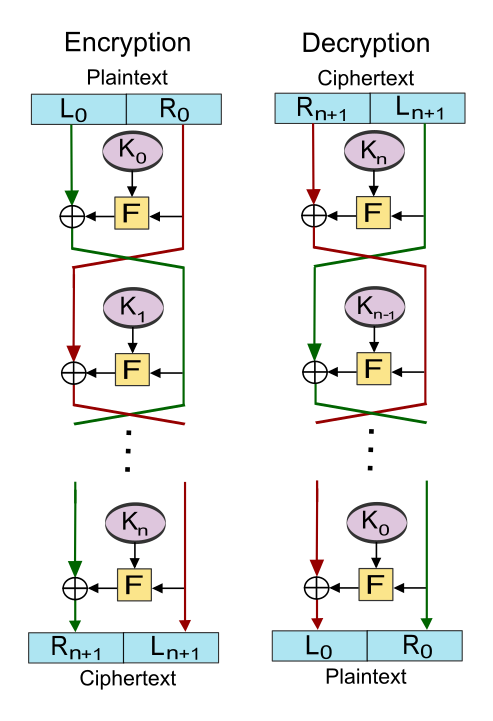
\includegraphics[width=.3\linewidth]{./493px-Feistel_cipher_diagram_en.svg.png}
            \caption{Diagram of feistel network cipher.}
        \end{center}
    \end{figure}

    The division of the plaintext into smaller blocks ensures that each block can be processed individually using the existing block encryption function $E$. To encrypt the last block, the Feistel network is employed. The Feistel structure divides the block into two equal-sized partitions, $L_0$ and $R_0$, each consisting of $k$ bits. The network then performs a specified number of rounds, applying a round function that operates on $L_j$ and $R_j$ to produce $L_{j+1}$ and $R_{j+1}$ for each round $j$. The final output of the Feistel network is the encrypted version of the last block, denoted as $b_{i+1}^*$.

    \vspace{.2cm} By combining the encryption of the preceding blocks using conventional block encryption modes and the encryption of the last block using the Feistel network, the proposed procedure achieves the desired size of the ciphertext.

    \section{Security Considerations}

    \vspace{.1cm}The security of the proposed procedure relies on the security properties of the block encryption function $E$ and the management of the encryption key. The underlying encryption algorithm must exhibit strong resistance against known cryptographic attacks, such as differential cryptanalysis, linear cryptanalysis, or related-key attacks. Additionally, the mode of operation used for encrypting the intermediate blocks should provide adequate security measures.

    \vspace{.2cm} The Feistel network, when properly designed and implemented, offers a robust cryptographic structure. It ensures that even if an attacker gains partial knowledge of the internal state or obtains intermediate values during encryption, the original plaintext remains secure.

    \vspace{.2cm} It is essential to consider key management and key size when extending block encryption. The key used in the original block encryption function $E$ should be of size $k$ and be securely generated and distributed. The Feistel network requires a separate key or key derivation mechanism to ensure the security of the extended encryption scheme. It could also be implemented as the extension of key generator used in encryption mode.

    \section{Points: 1/5}

\end{document}